\documentclass{amsart} 
\usepackage{amsmath}
\usepackage{verse}
\DeclareMathOperator*{\argmax}{arg\,max}
\DeclareMathOperator*{\argmin}{arg\,min}
\usepackage{graphicx}
\graphicspath{{./}}
\usepackage[fontsize=14pt]{scrextend}
\usepackage{hyperref}
\usepackage{csvsimple}
\usepackage{epigraph}
\title{People Everywhere Have Same Distribution on Religious Leader Influence}
\author{Zulfikar Moinuddin Ahmed}
\date{\today}
\begin{document}
\maketitle

The approval of religious leaders' influence in 44 countries showed remarkable stability in distribution.

% latex table generated in R 4.0.3 by xtable 1.8-4 package
% Wed Apr 14 10:46:24 2021
\begin{table}[ht]
\centering
\begin{tabular}{rrrr}
  \hline
 & x & sx & tf \\ 
  \hline
1 & 0.2938 & 0.0104 &  1 \\ 
  2 & 0.4322 & 0.0114 &  2 \\ 
  3 & 0.1764 & 0.0085 &  3 \\ 
  4 & 0.0976 & 0.0068 &  4 \\ 
   \hline
\end{tabular}
\caption{Influence of religious leaders} 
\end{table}

A helpful graphical display shows the tight bounds around the means.

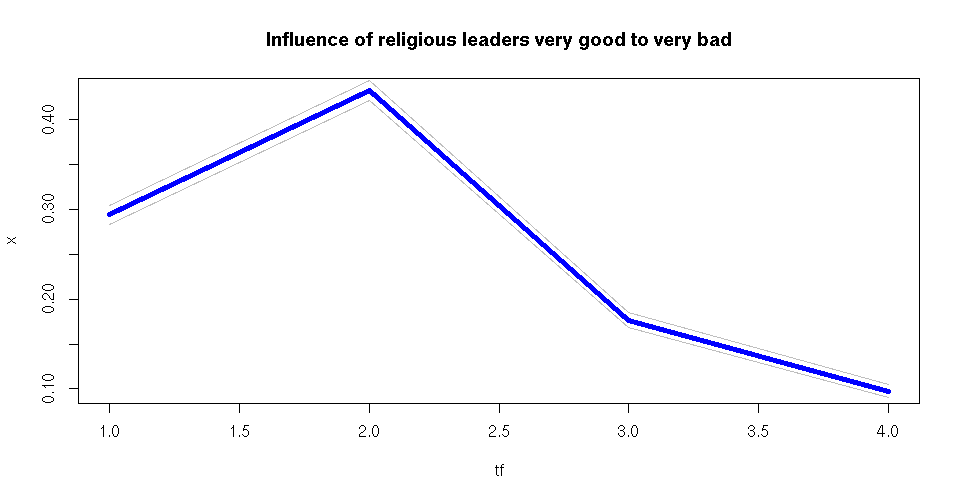
\includegraphics[scale=0.5]{relop.png}

\section{Surprise of the Result}

This result is extremely unexpected, because the religions represented in the countries is widely varying and yet there is a stability in the distribution of opinions about their influence that is quite uncanny.  We attribute this as well to Universal Human Nature feature.


\end{document}

